\documentclass[tikz]{standalone}
\usepackage{amsmath}
\usetikzlibrary{calc,arrows.meta,backgrounds}
\pagecolor[HTML]{171D2B}
\definecolor{aksen}{HTML}{F7B538}
\definecolor{teks}{HTML}{FFFFFF}
\definecolor{garis}{HTML}{94A3B8}

\begin{document}
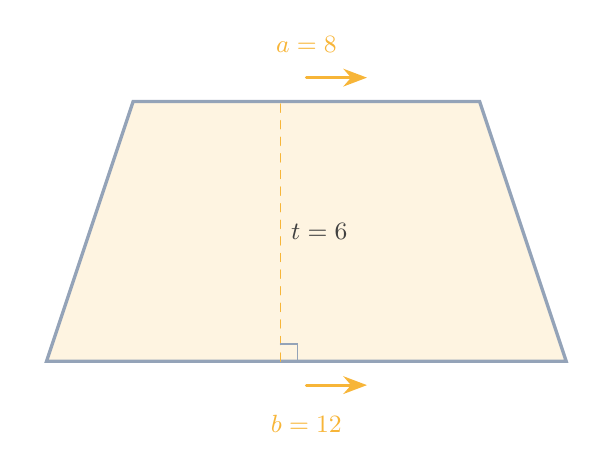
\begin{tikzpicture}[x=0.55cm,y=0.55cm,line cap=round,
  every node/.style={text=teks,font=\small}]

  \coordinate (A) at (0,0);
  \coordinate (B) at (12,0);
  \coordinate (C) at (10,6);
  \coordinate (D) at (2,6);

  \fill[aksen!15] (A) -- (B) -- (C) -- (D) -- cycle;
  \draw[very thick,garis] (A) -- (B) -- (C) -- (D) -- cycle;

  % tinggi
  \draw[dashed,aksen] ($(A)!0.45!(B)$) -- ++(0,6);
  \node[inner sep=1pt,outer sep=2pt,text=black!75] at ($(A)!0.45!(B)+(0.9,3)$) {$t=6$};

  % panah kesejajaran
  \draw[-{Stealth[length=3mm]},aksen,line width=1pt]
    ($(A)!0.5!(B)+(0,-0.55)$) -- ($(A)!0.5!(B)+(1.4,-0.55)$);
  \draw[-{Stealth[length=3mm]},aksen,line width=1pt]
    ($(D)!0.5!(C)+(0,0.55)$) -- ($(D)!0.5!(C)+(1.4,0.55)$);

  % label sudut siku di kaki tinggi
  \draw[garis] ($(A)!0.45!(B)+(0.4,0)$) -- ($(A)!0.45!(B)+(0.4,0.4)$) -- ($(A)!0.45!(B)+(0,0.4)$);

  \node[below=6pt] at (A) {$A$};
  \node[below=6pt] at (B) {$B$};
  \node[above right=2pt] at (C) {$C$};
  \node[above left=2pt] at (D) {$D$};
  \node[below=16pt,aksen] at ($(A)!0.5!(B)$) {$b=12$};
  \node[above=14pt,aksen] at ($(D)!0.5!(C)$) {$a=8$};
\end{tikzpicture}
\end{document}
